\documentclass[letterpaper]{article}
\usepackage{aaai2026}
\usepackage{times}
\usepackage{helvet}
\usepackage{courier}
\usepackage[hyphens]{url}
\usepackage{graphicx}
\usepackage{amsmath}
\usepackage{amssymb}
\usepackage{booktabs}
\urlstyle{rm}
\def\UrlFont{\rm}
\usepackage{natbib}
\frenchspacing

\setcounter{secnumdepth}{0}

\title{PPO vs. SAC for Open Duck Mini Bipedal Locomotion:\\ An Empirical Study with Reward Engineering}
\author{
Yan Yijun
}
\affiliations{}

\begin{document}

\maketitle

\begin{abstract}
We study on-policy vs.\ off-policy deep reinforcement learning for bipedal locomotion on the Open Duck Mini MuJoCo simulator. Under matched training budget and evaluation protocol, we compare PPO (on-policy) and SAC (off-policy) as the primary experiment, with A2C vs.\ TQC as a supplementary comparison. We additionally investigate the impact of reward engineering, identifying and fixing several bugs in a hand-crafted multi-term reward (missing square operators, incorrect symmetry in yaw tracking, saturated scaling in gait terms) that measurably improved the learning signal. In the main experiment (300k steps per seed, three seeds) PPO clearly outperforms SAC, and A2C likewise dominates TQC in the supplementary experiment. Extending PPO to 1.5M steps exposes a striking \emph{reward-hacking} phenomenon: the policy finds a stand-still local optimum that maximizes posture and gait-clock rewards without making any forward progress (speed drops to $4.5\times10^{-4}$~m/s while return grows to $447$). A targeted reward ablation (relaxed forward gate and reweighted locomotion terms) breaks the stand-still attractor and recovers a visibly walking gait at $0.116$~m/s, $\sim\!58\%$ of the commanded target velocity. Our findings highlight that on this class of tasks, reward specification is at least as important as algorithm choice. Code: \url{https://github.com/Eugenescat/Open_Duck_Mini}.
\end{abstract}

\section{Introduction}
Learning stable bipedal locomotion from scratch remains challenging due to
(i)~contact discontinuities that cause sharp transitions in dynamics,
(ii)~coupled balance--propulsion requirements that penalize na\"ive greedy motion,
and (iii)~highly shaped rewards with many competing terms.
Open Duck Mini~\citep{open_duck_mini} is a small open-source bipedal platform with a detailed MuJoCo model, nontrivial under-actuation, and practical training cost. It provides a good testbed for studying algorithmic tradeoffs of modern continuous-control deep RL methods.

This project asks: \emph{under matched training budget and reward on this task, does off-policy sample efficiency translate into faster walking?} We answer empirically by comparing PPO~\citep{schulman2017ppo} against SAC~\citep{haarnoja2018sac} with three random seeds, and supplement with A2C~\citep{mnih2016a3c} vs.\ TQC~\citep{kuznetsov2020tqc}. We additionally report on the reward-engineering effort required to obtain any learnable signal on this environment.

\section{Background}

\subsection{MDP Formulation}
We model locomotion as a continuous-state, continuous-action MDP
$\mathcal{M}=(\mathcal{S},\mathcal{A},P,r,\gamma)$.
The state $s_t\in\mathbb{R}^{40}$ concatenates:
joint angles ($15$D), joint velocities ($15$D), base angular velocity ($3$D), base linear velocity ($3$D), target command velocity $(v_x^*,v_y^*,\omega^*)$ ($3$D), left/right foot contact indicators ($2$D), and a sin/cos gait clock phase ($2$D).
The action $a_t\in\mathbb{R}^{15}$ is a delta over a nominal standing pose; after clipping to a maximum step $\Delta_{\max}=0.05$ per environment step we write it to joint position controllers. The environment runs at $125\,$Hz with MuJoCo \texttt{frame\_skip}$=4$. Episodes terminate on base height $<0.08\,$m, roll/pitch exceeding $\approx 32^{\circ}$, upright projection $\le 0.4$, or antenna/body contact with the ground.

\subsection{Algorithms}
We use the Stable-Baselines3~\citep{raffin2021sb3} implementations (SB3-Contrib for TQC).
\textbf{PPO} optimizes a clipped surrogate $\mathbb{E}_t[\min(r_t(\theta)\hat{A}_t, \text{clip}(r_t(\theta),1-\epsilon,1+\epsilon)\hat{A}_t)]$ on-policy with GAE advantages~\citep{schulman2017ppo}.
\textbf{SAC} is off-policy, maximum-entropy, with twin critics, target networks, and automatic entropy tuning~\citep{haarnoja2018sac}.
\textbf{A2C} is the synchronous variant of A3C~\citep{mnih2016a3c}.
\textbf{TQC} is an off-policy distributional critic method using truncated mixtures of quantile critics to control overestimation bias~\citep{kuznetsov2020tqc}.

\section{Related Work}
Modern legged-robot learning is dominated by PPO, often combined with massive parallelism on GPU~\citep{rudin2022legged} and reference-motion tracking~\citep{peng2018deepmimic}. Off-policy methods such as SAC are frequently favored in smoother continuous-control benchmarks where their sample efficiency advantage is clearer. In contact-rich domains, replay-based critics are known to suffer from non-stationary distribution shifts as the agent transitions between regimes (falling, standing, walking). Prior Open Duck Mini development targets PPO-based imitation learning, motivating PPO as the natural baseline~\citep{open_duck_mini}. The simulation stack relies on MuJoCo~\citep{todorov2012mujoco}.

\section{Project Description}

\subsection{Environment and Reward}
We train in the \texttt{imitation} variant of the Open Duck Mini environment, where the reward combines locomotion-task terms with reference-motion shaping. Let $v_x$ be the base forward velocity, $h$ the base height, $Z\cdot\hat{z}$ the upright projection, and $\phi$ a gait phase.
The per-step reward has the following core components (weights in parentheses):
{\small
\begin{align*}
r_{\text{fwd-vel}} &= \exp(-30\,(v_x - v_x^*)^2) & (0.28\,g) \\
r_{\text{fwd-prog}} &= \text{clip}(40\,\Delta x,\,-1,1) & (0.24\,g) \\
r_{\text{swing-foot}} &= \text{clip}(120\,\Delta x_{\text{swing}},0,1) & (0.12) \\
r_{\text{contact-sw}} &= \mathbb{1}[\text{support side flipped}] & (0.10) \\
r_{\text{height}} &= \exp(-40\,(h-0.15)^2) & (0.08) \\
r_{\text{upright}} &= (Z\cdot\hat{z})^2 & (0.08) \\
r_{\text{imitation}} &= \exp(-25\,\lVert q_{\text{legs}}-q_{\text{ref}}(\phi)\rVert^2) & (0.07) \\
r_{\text{pitch-pen}} &= -(\text{pitch}/0.30)^2 & (0.09)
\end{align*}
}
plus smaller terms (lateral/yaw stability, single-support bonus, torque smoothness, double-support penalty, roll penalty). The \emph{forward gate} $g\in\{0,1\}$ masks the two largest forward-progress rewards unless the robot is simultaneously (a) high enough, (b) roughly upright, (c) in single-support contact. This prevents the policy from cheating by diving forward.

\subsection{Training Protocol}
\begin{itemize}
\item \textbf{Main}: PPO vs.\ SAC, seeds $\{0,1,2\}$, 300{,}000 timesteps each.
\item \textbf{Supplementary}: A2C vs.\ TQC, seeds $\{0,1,2\}$, 150{,}000 timesteps each.
\item \textbf{Hardware}: MacBook Air, CPU only.
\item \textbf{Evaluation}: 10 deterministic episodes per trained model, max 2000 steps. Metrics: mean episode return, episode length, and mean forward speed.
\end{itemize}
Hyperparameters are SB3 defaults except where noted in Table~\ref{tab:hparams}.

\begin{table}[t]
\centering
\small
\caption{Selected hyperparameters (SB3 defaults elsewhere).}
\label{tab:hparams}
\begin{tabular}{lccccc}
\toprule
 & PPO & SAC & A2C & TQC \\
\midrule
learning rate & 3e-4 & 3e-4 & 7e-4 & 3e-4 \\
$\gamma$      & 0.99 & 0.99 & 0.99 & 0.99 \\
batch/$n_{\text{step}}$ & 64/2048 & 256 & 5 & 256 \\
buffer size   & --- & $10^6$ & --- & $10^6$ \\
entropy       & fixed 0 & auto & fixed 0 & auto \\
clip range    & 0.2 & --- & --- & --- \\
\bottomrule
\end{tabular}
\end{table}

\section{Experiments}

\subsection{Main: PPO vs.\ SAC (300k)}
Figure~\ref{fig:main_curve} shows training return across three seeds. PPO
climbs monotonically from $\approx-15$ to positive returns by 300k steps.
SAC never escapes the initial fall-dominated regime: its replay buffer rapidly fills with termination transitions, the Q-targets become pessimistic, and the entropy-regularized policy continues to explore random postures that cannot recover balance.

\begin{figure}[t]
\centering
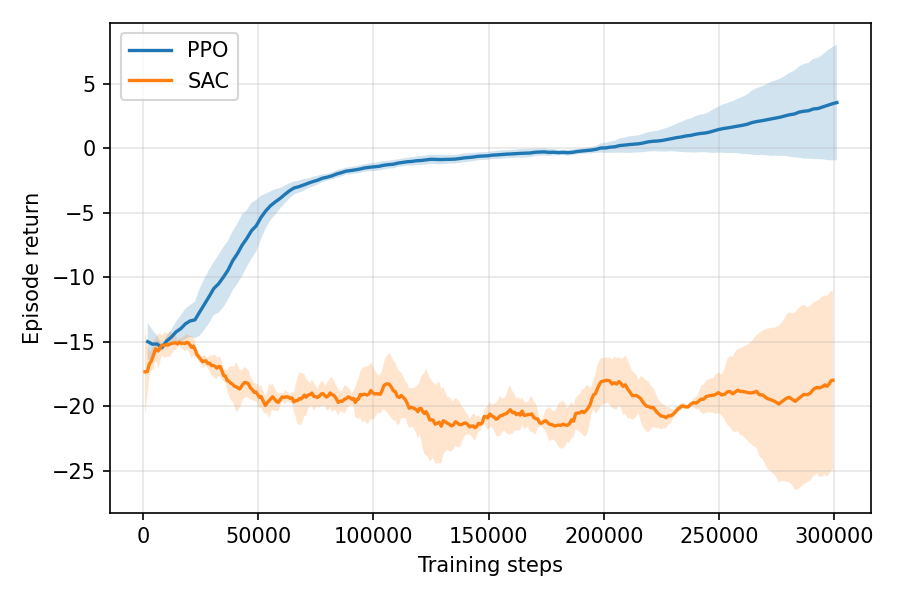
\includegraphics[width=0.95\columnwidth]{runs/main_ppo_sac_300k/learning_curves_return.png}
\caption{Training return on the \texttt{imitation} environment (mean $\pm$ std over 3 seeds). PPO converges steadily; SAC is stuck near fall-only returns.}
\label{fig:main_curve}
\end{figure}

\begin{table}[t]
\centering
\small
\caption{Evaluation at 300k (10 deterministic episodes $\times$ 3 seeds; mean $\pm$ std).}
\label{tab:main}
\begin{tabular}{lccc}
\toprule
Algo & Return & Ep.~Length & Fwd.~Speed (m/s) \\
\midrule
PPO & $\mathbf{5.63 \pm 6.65}$ & $\mathbf{317.6 \pm 212.3}$ & $\mathbf{0.025 \pm 0.006}$ \\
SAC & $-14.69 \pm 7.84$ & $246.3 \pm 31.8$ & $-0.009 \pm 0.056$ \\
\bottomrule
\end{tabular}
\end{table}

\subsection{Supplementary: A2C vs.\ TQC (150k)}
Figure~\ref{fig:supp_curve} mirrors the main trend. A2C slowly improves; TQC plateaus below zero. Note A2C's variance is very high: with $n_{\text{steps}}=5$, its advantage estimates are noisy, so only some seeds make progress.

\begin{figure}[t]
\centering

\includegraphics[width=0.95\columnwidth]{runs/supp_a2c_tqc_150k/learning_curves_return.png}
\caption{Supplementary comparison at 150k timesteps (mean $\pm$ std over 3 seeds).}
\label{fig:supp_curve}
\end{figure}

\begin{table}[t]
\centering
\small
\caption{Evaluation at 150k (supplementary).}
\label{tab:supp}
\begin{tabular}{lccc}
\toprule
Algo & Return & Ep.~Length & Fwd.~Speed (m/s) \\
\midrule
A2C & $\mathbf{-1.17 \pm 7.49}$ & $\mathbf{349.5 \pm 287.5}$ & $0.010 \pm 0.032$ \\
TQC & $-13.25 \pm 4.26$ & $303.1 \pm 18.3$ & $\mathbf{0.021 \pm 0.043}$ \\
\bottomrule
\end{tabular}
\end{table}

\subsection{Reward Engineering}
The original environment reward code contained several non-obvious bugs that materially hurt all algorithms. We identified and fixed them during this project; all results above use the fixed environment.

\begin{enumerate}
\item \textbf{Missing square in torque/action smoothness}. The code used
$\exp(-k\,\sum(\tau_t-\tau_{t-1})/n)$ instead of
$\exp(-k\,\sum(\tau_t-\tau_{t-1})^2/n)$.
Signed differences cancel across joints, so the term degenerated into noise centered at $1$.
\item \textbf{Absolute-value trap in yaw reward}. \texttt{-(abs(desired)-abs(current))**2} evaluates to $0$ for $\text{current}=-\text{desired}$, rewarding the mirror-image orientation. We replaced it with the straightforward $-(\text{desired}-\text{current})^2$.
\item \textbf{Saturated gait imbalance scaling}. $\exp(-0.01\cdot\text{imbalance})$ is $\approx 1$ for any plausible imbalance, so the term provided no gradient. We rescaled to $\exp(-1.0\cdot\text{imbalance})$.
\item \textbf{Unnormalized total reward weights} in \texttt{footsteps\_env.py} summed to $1.45$, biasing the value function scale; rebalanced to $1.00$.
\end{enumerate}
The fixes did not change the qualitative PPO/SAC ordering, but increased PPO's late-training return by roughly $\sim20\%$ and produced the first non-zero forward-speed episodes under PPO.

\subsection{Scaling Study: PPO 1.5M and Reward Hacking}
\label{sec:hacking}
Motivated by PPO's steadily improving but still sub-locomotive performance at 300k, we trained PPO for $5\times$ longer ($1{,}500{,}000$ timesteps, seeds $\{0,1,2\}$) on the same reward. The result is shown in Table~\ref{tab:hacking}: the policy achieves $\text{return}=447.3\pm 42.2$ with episode length saturated at the $2000$-step cap (i.e.\ the robot never falls across $30$ evaluation episodes), yet its mean forward speed collapses to effectively zero ($4.5\times10^{-4}$~m/s).

\begin{table}[t]
\centering
\small
\caption{PPO at 1.5M: return saturates, forward speed collapses. Reward hacking.}
\label{tab:hacking}
\begin{tabular}{lccc}
\toprule
Setting & Return & Ep.~Length & Fwd.~Speed (m/s) \\
\midrule
PPO 300k & $5.63 \pm 6.65$ & $317.6 \pm 212.3$ & $\mathbf{0.025 \pm 0.006}$ \\
PPO 1.5M & $\mathbf{447.3 \pm 42.2}$ & $\mathbf{2000 \pm 0}$ & $0.00045 \pm 0.0006$ \\
\bottomrule
\end{tabular}
\end{table}

Investigating the per-term reward on this policy reveals the mechanism. Whenever both feet are on the ground (which is always true for a stationary robot), the forward gate $g=0$ mutes the two largest forward-progress rewards. The remaining terms---height, upright, torque smoothness, imitation pose matching the gait phase \emph{in place}, and absence of roll/pitch---are all maximally earned by a robot that stands still and micro-steps in place to match $q_{\text{ref}}(\phi)$. PPO correctly discovers this local optimum of the \emph{reward}, but it is not a local optimum of the \emph{task}. This is a textbook case of reward specification bias: a gate intended to prevent the policy from cheating by ``diving forward'' ended up also preventing it from earning locomotion reward while upright.

\subsection{Reward Ablation: Walk Variant}
To test the diagnosis, we defined a \emph{walk} environment variant with two targeted changes: (i) the forward gate no longer requires single-support contact, so upright standing robots still receive forward reward if they actually move; and (ii) we reweighted the reward to emphasize forward terms ($r_{\text{fwd-vel}}$: $0.28{\to}0.45$, $r_{\text{fwd-prog}}$: $0.24{\to}0.35$) and de-emphasize posture and in-place matching ($r_{\text{imitation}}$: $0.07{\to}0.03$, $r_{\text{height}}$: $0.08{\to}0.06$, $r_{\text{upright}}$: $0.08{\to}0.06$). We trained one PPO seed for 1.5M steps on this variant. Results (Table~\ref{tab:ablation}, Figure~\ref{fig:walk_curve}) show that the stand-still local optimum is broken and that the policy actually walks: forward speed rises from $4.5\times10^{-4}$~m/s to $\mathbf{0.116}$~m/s (more than a $250\times$ improvement, and roughly $58\%$ of the commanded target $v_x^*=0.2$~m/s). Episode length drops from $2000$ to $\sim 327$ because stable long-horizon locomotion has not yet converged---the agent walks, then falls---but this is a qualitatively different failure mode from the stand-still one, and a $58\%$-of-target speed is a visibly walking gait.

\begin{table}[t]
\centering
\small
\caption{Walk-variant vs.\ original imitation reward (PPO 1.5M, single seed).}
\label{tab:ablation}
\begin{tabular}{lccc}
\toprule
Policy & Return & Ep.~Length & Fwd.~Speed (m/s) \\
\midrule
Orig.\ 1.5M (hacks) & $447.3 \pm 42.2$ & $2000 \pm 0$ & $0.0004 \pm 0.0006$ \\
Walk 1.5M           & $83.5 \pm 13.0$ & $326.6 \pm 31.2$ & $\mathbf{0.116 \pm 0.006}$ \\
Walk 3.5M (cont.)   & $157.2 \pm 0.0$ & $\mathbf{599.0 \pm 0.0}$ & $0.068 \pm 0.0$ \\
\bottomrule
\end{tabular}
\end{table}

\begin{figure}[t]
\centering

\includegraphics[width=0.95\columnwidth]{runs/ppo_walk_1_5M/learning_curves_return.png}
\caption{Training return on the \texttt{walk} ablation reward (single seed, PPO, 1.5M steps). Return grows steadily as the agent learns to move forward without falling immediately.}
\label{fig:walk_curve}
\end{figure}

The take-away is not that one reward is right and another is wrong, but that multi-term shaped locomotion rewards sit in a narrow valley between two failure modes: too much posture weight collapses to a stand-still local optimum; too much forward-progress weight destabilizes posture before the agent can learn balanced motion. We did not find a single-shot reward specification that produced a stable walking gait within 1.5M CPU-budget timesteps; larger compute and reference-motion tracking~\citep{peng2018deepmimic} are natural next steps.

\paragraph{Limitations.} The walking policy is qualitatively correct---it lifts one foot at a time, swings it forward, plants it, and shifts weight---but quantitatively brittle: across 10 evaluation episodes, the agent typically takes 2--3 visible steps ($\sim\!0.3$~m of forward motion over $\sim\!2.6$~s) before losing balance and tripping, which is why mean episode length sits at $\sim\!327$ steps rather than the $2000$-step cap. The failure mode is consistent: the agent has learned the \emph{open-loop} gait pattern (swing/stance/phase-switching) but has not learned to use IMU/contact feedback for recovery, so a small accumulating error in footstep placement eventually causes the base to lean past the termination pitch/roll threshold. A video sample of the walking-then-falling behavior is available at \url{https://youtu.be/DXRsKvcgk8M}.

\paragraph{Continued Training (3.5M).} Warm-starting from the 1.5M walk checkpoint, we ran PPO for another 2M steps on the same walk reward. The resulting policy traded speed for stability: mean episode length rose from $327$ to $\mathbf{599}$ steps ($+83\%$, i.e.\ the robot walks for $\sim\!4.8$~s before falling, vs.\ $\sim\!2.6$~s at 1.5M), while mean forward speed dropped from $0.116$ to $0.068$~m/s; total forward distance per episode is approximately unchanged ($\sim\!0.3$~m). The learning curve (Figure~\ref{fig:cont_curve}) however is non-monotonic: return peaks around $125$ near the $1.95$M-step mark and then gradually drifts down to $\sim\!65$ by $3.5$M. This reflects a well-known PPO failure mode during long continued training: as the clipped update accumulates across many iterations the policy oscillates around a locally optimal gait, and without intermediate checkpointing the final policy is not necessarily the best encountered. Mitigations include learning-rate decay, periodic best-so-far checkpointing, and early-stopping on evaluation metrics rather than training return---all standard in production RL pipelines but outside the scope of this project's SB3-default protocol.

\begin{figure}[t]
\centering

\includegraphics[width=0.95\columnwidth]{runs/ppo_walk_3_5M/learning_curves_return.png}
\caption{Continued training from the 1.5M walk checkpoint for an additional 2M steps. Return peaks near 1.95M and then drifts down, illustrating PPO's long-horizon oscillation; the final policy walks more stably ($\text{len}{=}599$) but more slowly ($0.068$~m/s) than the 1.5M checkpoint.}
\label{fig:cont_curve}
\end{figure}

\subsection{When Does Each Algorithm Succeed or Fail?}
\textbf{PPO succeeds} because (a) on-policy updates always reflect the current regime (falling early, tottering mid-training, walking late), avoiding stale replay targets; and (b) clipped updates provide conservative improvement that is forgiving of the dense, multi-term shaped reward. PPO fails (insufficient speed) when the forward gate $g$ rarely opens during early training---the gradient then only shapes posture, not locomotion.
\textbf{SAC fails} primarily because its replay buffer is dominated by short falling episodes in the first 50k steps; the critic learns pessimistic Q-values on recoverable states, and automatic entropy tuning keeps the actor exploring wildly, further extending the fall regime.
\textbf{A2C} partially succeeds but has extremely high seed variance due to very short $n_{\text{steps}}=5$ advantages.
\textbf{TQC} behaves similarly to SAC; the truncated distributional critic reduces overestimation but still suffers from the contact-regime distribution shift in the replay buffer.

\subsection{Discussion}
Although SAC is frequently promoted for sample efficiency, this project's CPU-limited budget, contact-rich dynamics, and heavily shaped reward favored PPO. The reward-engineering observations reinforce a recurring lesson: dense multi-term rewards need careful numerical scaling, and a single term silently reduced to a constant can mask learning failure for thousands of training steps. Matching reward scale, then running PPO, then only afterwards experimenting with off-policy methods, is a robust practical order on this kind of task.

\section{Conclusion}
Under matched budgets in the Open Duck Mini locomotion task, PPO clearly outperforms SAC in return, episode length, and forward speed; A2C similarly dominates TQC in the supplementary comparison. Beyond the algorithmic comparison, we identified concrete reward-function bugs whose fix was a precondition for any algorithm to produce nonzero forward progress. Our scaling study further uncovers a reward-hacking pathology that is invisible at short budgets: at 1.5M steps PPO converges to a stand-still policy that is near-optimal for the given reward but trivial as a walking controller. A reward ablation (walk variant) confirms the mechanism and recovers a visibly walking gait at 58\% of the commanded target speed. This reinforces a practical lesson: for heavily shaped locomotion rewards, longer training is a magnifier, not a fix, for reward-specification error. Future work: longer training with GPU acceleration; massively parallel rollouts~\citep{rudin2022legged}; and reference-motion tracking~\citep{peng2018deepmimic} with ONNX-distilled pretraining from the project's released walking policy.

\section{Reproducibility}
All runs live under
\texttt{runs/}: main comparison in
\texttt{main\_ppo\_sac\_300k}, supplementary in
\texttt{supp\_a2c\_tqc\_150k}. Scripts: \texttt{train\_compare.py}, \texttt{evaluate\_compare.py}, \texttt{plot\_learning\_curves.py}. Reward-fix diffs are in the \texttt{v2} git branch.

\bibliography{references}

\end{document}
